%%%%%%%%%%%%%%%%%%%%%%%%%%%%%%%%%%%%%%%%%%%%%%%%%%%%%%%%%%%%%%%%%%%%%%%%%%%%%%%%
%2345678901234567890123456789012345678901234567890123456789012345678901234567890
%        1         2         3         4         5         6         7         8

\documentclass[letterpaper, 10 pt, conference]{ieeeconf}  % Comment this line out
                                                          % if you need a4paper
%\documentclass[a4paper, 10pt, conference]{ieeeconf}      % Use this line for a4
                                                          % paper

\IEEEoverridecommandlockouts                              % This command is only
                                                          % needed if you want to
                                                          % use the \thanks command
\overrideIEEEmargins
% See the \addtolength command later in the file to balance the column lengths
% on the last page of the document



% The following packages can be found on http:\\www.ctan.org
%\usepackage{graphics} % for pdf, bitmapped graphics files
%\usepackage{epsfig} % for postscript graphics files
%\usepackage{mathptmx} % assumes new font selection scheme installed
%\usepackage{times} % assumes new font selection scheme installed
%\usepackage{amsmath} % assumes amsmath package installed
%\usepackage{amssymb}  % assumes amsmath package installed

\title{\LARGE \bf
Evaluating Style Transfer
}
\author{Peter W. Kong}
%\author{ \parbox{3 in}{\centering Huibert Kwakernaak*
%         \thanks{*Use the $\backslash$thanks command to put information here}\\
%         Faculty of Electrical Engineering, Mathematics and Computer Science\\
%         University of Twente\\
%         7500 AE Enschede, The Netherlands\\
%         {\tt\small h.kwakernaak@autsubmit.com}}
%         \hspace*{ 0.5 in}
%         \parbox{3 in}{ \centering Pradeep Misra**
%         \thanks{**The footnote marks may be inserted manually}\\
%        Department of Electrical Engineering \\
%         Wright State University\\
%         Dayton, OH 45435, USA\\
%         {\tt\small pmisra@cs.wright.edu}}
%}

% \author{Huibert Kwakernaak$^{1}$ and Pradeep Misra$^{2}$% <-this % stops a space
% \thanks{*This work was not supported by any organization}% <-this % stops a space
% \thanks{$^{1}$H. Kwakernaak is with Faculty of Electrical Engineering, Mathematics and Computer Science,
%         University of Twente, 7500 AE Enschede, The Netherlands
%         {\tt\small h.kwakernaak at papercept.net}}%
% \thanks{$^{2}$P. Misra is with the Department of Electrical Engineering, Wright State University,
%         Dayton, OH 45435, USA
%         {\tt\small p.misra at ieee.org}}%
% }
\usepackage{textcomp}
\usepackage{hyperref}
\usepackage{graphicx}

\begin{document}



\maketitle
\thispagestyle{empty}
\pagestyle{empty}


%%%%%%%%%%%%%%%%%%%%%%%%%%%%%%%%%%%%%%%%%%%%%%%%%%%%%%%%%%%%%%%%%%%%%%%%%%%%%%%%
\begin{abstract}

This project formalizes the problem of evaluation of monolingual sequence to sequence style transfer models and explores improvements on the state of the art metrics.

\end{abstract}


%%%%%%%%%%%%%%%%%%%%%%%%%%%%%%%%%%%%%%%%%%%%%%%%%%%%%%%%%%%%%%%%%%%%%%%%%%%%%%%%


\section{Introduction}
                
        
Style identification is the identification of style in a text passage by an automated process, often a language model. Generative models can generate text in one or more styles, given content and style parameters. Style identification has proven utility in applications like author identification (Houvardas). Yet, while much research has focused on semantic transfer from one human language to another, there has been little attention paid to intra-lingual style transfer. Intra-lingual style transfer affords many interesting applications: authorship obfuscation, text simplification, and style enhancement, to name a few.

The existing literature on style transfer uses a combination of BLEU scores, perplexity [Ficler], black box neural classifiers, and manual labeling to evaluate the quality of a transfer. Each of these has serious problems (see Section 3)


This paper\textquotesingle s objectives are three-fold:
\begin{itemize}
    \item Identify characteristics desirable in a style transfer evaluation metric
    \item Formalize the evaluation objective
    \item Explore a specific approach and discuss results
\end{itemize}
          

\section{Related work}

There is active research in style transfer. Ficler uses fixed, human- intelligable stylistic parameters like ’length’ and ’sentiment’, which can be extracted from specific training data with heuristics. They use perplexity as an evaluation metric.
\\ 

[Fu, et al.] addresses the problem of learning style transfer without the use of parallel corpora, using style embeddings (a previous work) and an auto-encoder model with multiple decoders. Attempts are made to improve evaluation metrics, but they do not appear to improve on human judgment and black-box classifiers. Example outputs from models are hard to visualize/express in a relatable way.
\\ 

[Hu] seeks to generate realistic (English) sentences using a VAE in a wake-sleep configuration. Semantic and stylistic signals can be injected to coerce specific meaning and styles.
Outperforms stated previous work: a semi-supervised VAE (Kingma 2014). Hu reaches about 83pct sentiment classification accuracy, although performance varies greatly with datasets used. Hu's metric is label accuracy using external (i.e. blackbox) sentiment classifiers.
\\ 

[Prabhumoye]'s proposed model creates a style-agnostic representation of an English input sentence using A->B then B->A neural machine translators, with the objective of style transfer with minimal semantic drift. A style-specific transformation step adds specific style to the style-agnostic representation. This paper confirms that BLEU and ROUGE metrics are not suitable for capturing meaning.

\section{Criticism of existing style transfer metrics}
In this section we comment on existing metrics used to evaluate style transfer (or similar tasks).
\begin{itemize}
  \item{ Perplexity and BLEU}
  \\
  Perplexity, according to [Jurafsky] is the the normalized inverse probability of a test set, formalized as:
  \\
  \\
  $Perplexity(W) $ $=$ $\frac{1}{P(w_1 \ldots w_n)}^{\frac{1}{N}}$
  \\
  \\
  This metric is quite intuitive, simple, and portable. However, it suffers significant failures when evaluating across styles that use different words or word orderings. Consider this example inter-style sentence alignment:\\
  \\
  (Reference) Mary ate her cheeseburger.\\
  (Candidate A) A meal was eaten by Mary.\\
  (Candidate B) Mary said that Bob ate his cheeseburger but I think she's lying.\\
  \\
  Assume, reasonably, that (A) and (B) are both drawn from the same style corpus, and (C) is not: (A) and (B) are both concise and factual, while C uses indirect voice and a narrative effect.
  \\
  Candidate (B) will be heavily penalized because P(meal), P(was), P(A), and P(by) are all equal to zero.  The perplexity of (B) as compared with (A) will be high, since the metric accounts for specific words, not semantics or style. In contrast, perplexity will value (C)'s word overlap with (A), even though the overlapped words "ate" and "cheeseburger" are attached to different subjects.
  \\
  For the same reasons, the BLEU score is incorrectly penalizes candidates that express the same style and concepts, but with different words. \\

  \item{Neural Models}\\ As mentioned in Section 2, neural net classifiers are heavily used in sequence to sequence evaluation (including in style transfer), but they suffer poor explanatory power due to their composition of usually immense weight vectors that are not individually attached to human intelligable concepts. [Li, et al.] and others have attacked this problem with some success. However, achievements are still modest and tend to explain predictions row-by-row, rather than explaining the classifier as a whole. \\

  \item{Manual evaluation}\\
  Manual evaluation in theory provides great results, and indeed the majority of research in style transfer employs it so some degree. However, manual evaluation is obviously intractible for large amounts of training data. It is also subjective with respect to the human evaluators.
\end{itemize}

\section{Formalizing the problem}
  \subsection{problem formalization} We formalize the style transfer problem as:
    Given:
    \begin{itemize}
      \item a style transfer model $M_{AB}$ that attempts to transfer an input sentence in style A to style B
      \item a candidate output sentence from $M_{AB}$:  $x_{AB}^i$
      \item a reference sentence and score pair $R_{AB}^i ; y_i$ that is scored in a range of $[0,1]$ by a trusted external source
    \end{itemize}

  The evaluation metric E($x_{AB}^i$, $R_{AB}^i$) will output a score.A successful metric E will output a score $\hat{y}$, where $|y-\hat{y}|$ is minimized. Some variations on this loss function are detailed later.
  \subsection{Desired Evaluation metric traits}
      After reviewing the pros and cons of various evaluation metrics in the current literature, we distilled four desirable traits in an evaluation metric.
    \begin{itemize}

      \item The ideal metric $E()$ should be accurate. More precisely, it should track ground truth values closely. When the ground truth score for $x_{AB}^i$ is low, E($x_{AB}^i$, $R_{AB}^i, y_i$) should also be low. Likewise for high ground truth scores.
      \item $E()$ should be intuitive. It is common for research tasks to use [TODO: add reference] LSTM classifiers to evaluate style transfer (when, of course, human scores are not sufficiently available). While some of these neural classifiers achieve reasonable accuracy, their explanatory power is quite low. Humans cannot easily draw intuitions from the weight matrices of neural layers.
      \item $E()$ speed should be reasonable. We define this having a run time that is linear in the input data.
      \item $E()$ relies only on $X$, $R$, $Y$. This allows $E()$ to be portable between experiments and corpora.
      \item If $E()$ evaluates content in addition to style, it should do so independently
      We quickly realized that an improvement on the existing metrics required an ensemble of multiple submetrics.
    \end{itemize}
  \subsection{Discussion of exploratory paths} 
  With these traits in mind, we avoided including neural network, or other 'black box' classifiers in our evaluator. Instead, we focused on simple linear classifiers with intuitive engineered features. 


\section{Experiment setup}
  
  \subsection{Data}
  Experimental data was draw from Coco Xu's Shakespeare dataset. This dataset is drawn from two distinct sources: Shakespeare's original play scripts, and Sparknote's modernized versions. Sentences are aligned, so that the same sentence may be accessed simultaneously in both styles.
  All aligned sentences from the Shakespeare dataset were used, from the following plays:\\ \\ 'othello', 'antony-and-cleopatra', 'asyoulikeit', 
                       'errors', 'hamlet', 'henryv', 'juliuscaesar', 'lear', 'macbeth', 
                       'merchant', 'msnd', 'muchado', 'richardiii', 'romeojuliet', 
                       'shrew', 'tempest', 'twelfthnight'
\\ \\
  42,000 parallel sentences in total.
\\
  The topics encompass a wide variety of content and sentiment: comedies, tragedies, histories, although it is important to note that they are all written in the screenplay format. While this is an amazing corpus to work with, there are some natural limitations.

  Here are some examples of parallel aligned sentences. As you can see, differences in percieved style can vary significantly from passage to passage (original style on the left):


  \begin{table}[h]
    \caption{Aligned Text Examples}
    \label{table_example}
    \begin{center}
      \begin{tabular}{| p{3.5cm}  | p{3.5cm} |}
      \hline
      What's the matter, lieutenant? & What's the matter, lieutenant?\\
      \hline
      Tell me this, I pray: Where have you left the money that I gave you? & Answer me this, please: where's the money I gave you?\\
      \hline
      Lucius, who's that knocking? & Lucius, who's that knocking?\\
      \hline
      Gentlemen, forward to the bridal dinner. & Gentlemen, on to the bridal dinner.\\
      \hline
      \end{tabular}
    \end{center}
  \end{table}


The original sentences were automatically assigned a "class 1" label, and the sparknotes sentences a "class 2" label, this generating a classical supervised learning dataset with "gold" labels.

This dataset was randomly shuffled by sentence pair, preserving style-to-style alignments. 70pct of corpus was designated the train set, 20pct the validation set, and 10pct the holdout test set.
 
We experimented with a variety of models. However, the choice of experiments was guided by our evaluator design ideals (see previous section).

\subsection{Early Exploration - NER and BLEU}
We attempted to use NER scores as well, but found that they provided almost no predictive power even between content-aligned inter-style sentence pairs. And of course, using NER in a non-aligned context reduces portability. Furthermore, even if NER could be configured to yield predictive power, it adds a distracting content signal into the evaluator, violating one of our ideal traits.
\\ \\

We wanted to employ BLEU scoring as a sub-metric. To crudely abstract content from style in the Shakespeare dataset, we aggregated BLEU scores on randomized sentence pairs in three experiments: pairs drawn from Style A, pairs drawn from Style B, and pairs drawn from Styles A and B.

We hypothesized that if BLEU scores computed from same-style pairs were higher than inter-style, BLEU might differentiate between styles. Disappointingly, BLEU was not up to the task:

\begin{table}[h]
  \caption{Content-agnostic BLEU scoring}
  \label{table_example}
  \begin{center}
    \begin{tabular}{| p{2cm}  | p{2cm} |  }
    \hline
    Same-style, A & .016 \\
    \hline
    Same-style, B & .021\\
    \hline
    Inter-style & .017\\
    \hline
    \end{tabular}
  \end{center}
\end{table}



\subsection{Feature Engineering}
We used a total of of 1645 features in our final model, all human-intelligible.

Drawing from insight from Strunk and White's "The Elements of Style", we tracked the counts of the following punctuation marks in each sentence of each style: 
\\
\\
 : ; ' ( ... !
\\
\\
We constructed the remainder of the features from POS tagging and dependency parsing.
POS features were generated by the Spacy POS tagger, trained on a standard web corpus. We found the tagger to be quite accurate, even on the relatively ancient Shakespearean corpus. Example:\\
\\
"Go bid the priests do present sacrifice And bring me their opinions of success"\\
\\

\begin{table}[h]
  \caption{POS tagging}
  \label{table_example}
  \begin{center}
    \begin{tabular}{| p{2cm}  | p{2cm} | }
      \hline
      Go&VERB  \\  
      \hline
      bid&VERB\\ 
      \hline
      the&DET   \\
      \hline
      priests&NOUN \\
      \hline
      do&VERB   \\
      \hline
      present&ADJ  \\
      \hline
      sacrifice&\\
      \hline
      And&CCONJ \\
      \hline
      bring&VERB  \\
      \hline
      me&PRON   \\
      \hline
      their&ADJ    \\
      \hline
      opinions&NOUN  \\
      \hline
      of&ADP    \\
      \hline
      success&NOUN \\
      \hline
    \end{tabular}
  \end{center}
\end{table}

We also used adjective-noun ratios and adverb-verb ratios as separate features.

The last grouping of features, representing the majority, were one-hot POS sequence features. For example, this sentence: 
\\
\\
"A sleep that ends all the heartache."
\\
\\
would result in the feature "NOUN\textunderscore VERB\textunderscore NOUN" acquiring the value $1$, and "VERB\textunderscore NOUN" acquiring the value $0$. Note that we ignored all parts of speech except nouns, verbs, and conjunctions. We also truncated sequence features to a cardinality of 7 to prevent feature explosion. We found no accuracy improvement past this cardinality.


\subsection{Models}
We reviewed linear classification models that had good classification ability as well as the ability to output probability distributions of class predictions, rather than just the binary predictions.

    \begin{itemize}
      \item{Multinomial Naive Bayes} \\
      MNB has the ability to predict probabilities, which, while less helpful given our binary labeled data set, would be quite helpful in further verification of the evaluator for a future, ranged labeled dataset. With this in mind, we made the assumption that our binary training data labels were actually 100pct-weighted probability values. 
      \item{SVM}\\
      SVM also has the ability to predict probabilities and handles reasonably large numbers of one-hot features well.
    \end{itemize}
 

  \section{Results}
    \begin{table}[h]
      \caption{Model Performance}
      \label{table_example}
      \begin{center}
        \begin{tabular}{| p{2cm}  | p{2cm} | | p{2cm} }
        \hline
        Model & Validation Brier Score & Test-set Accuracy\\
        \hline
        SVM, all features, all plays & .614 & .696\\
        \hline
        TODO & add addl'l experiments & TODO \\
        \hline
        \end{tabular}
      \end{center}
    \end{table}

  \section{Analysis}
  We found that SVM, with all final features present, yielded the best classification accuracy across all models tried. Test set accuracy only decreases slightly from validation set accuracy. Thus, we are confident that overfitting is not a serious issue. We attribute close results to a large dataset and use of regularization within the SVM model.

  While the best evaluator was trained on the entire dataset we found that gains in accuracy began to level off around [TODO: add performance graph here]
  \\
  Evaluators should be quite accurate if they are to judge other models. Unfortunately, at 60pct accuracy we consider this evaluator a failure. \\
  \\
  It's worth noting that the evaluator made most of it's mistakes in misidentifying 'modern' sentences as 'original'.

  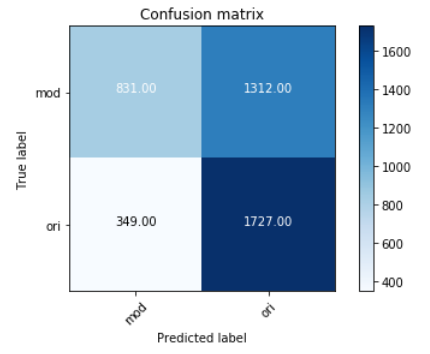
\includegraphics[scale=.5]{confmat.png}

  Without additional parallel style data, it is difficult to anticipate how the model will perform on non-Shakespearean datasets.

  We estimate that a significant amount of accuracy loss is attibutable to the binary nature of the dataset gold labels. Additional parallel corpora (from authors besides Shakespeare) with scalar rather than binary gold labels would undoubtedly guide use towards a better performing evaluator. Unfortunately, these parallel style corpora are virtually nonexistent.
  \\
  \\
  Cherry-picking intuition-guided features to engineer adds a subjective element to our evaluator, which is responsible for loss in accuracy, to a degree that is difficult to measure precisely. Doubtless, additional features exist that would improve accuracy.

  \subsection{Hyperparameter tuning}
    After experimenting with using RBF and polynomial kernels, we found that a linear kernel yielded the best result.


    Since this is an evaluation metric, it's important to strive for a non-binary output that closely tracks gold scoring along the entire range of possible values (i.e. 0 to 1)..\\
    Our best model, Multinomial Naive bayes with (XXX features) underperformed our intuition-driven expectations.


  \subsection{Acknowledged shortcomings}
  Assumption of evenly distributed class (style) priors. This is not a portable assumption. \\ \\The way forward will be to either prove evaluator success with heuristically seeded priors, or require the injection of class priors from each project's dataset. \\ \\
We only used one dataset, the Shakespeare dataset. It is simplistic to assume that Sparknotes data resembles a single human author's. It probably resembles other business objectives, like truncation.
\\
\\
  We assumed that each style's class prior probability was 50pct for the multinomial Naive Bayes models. While this was true of our dataset, it of course does not always hold. Future models with unknown class priors will have to account for this fact, perhaps by using stochastic priors.
\section{Future work}
[TODO: expand]
Expand approach to handle passages larger than single sentences\\

How do we deal with fluidity and overlapping between styles, or shifting style boundaries?\\

We assumed Style-author hypothesis: That an author always writes in the same style. This is probably not always the case. Do we tackle this issue by including author identification as a sub-metric in a future evaluator?


...
\section{Conclusions}
We hope that we have motivated the need for a better style transfer metric, and that our problem formalization will be helpful in future work. Unfortunately, our strategy of maximizing explanatory power through human-intelligible engineering features resulted in disappointing accuracy results in our best performing model, a Support Vector Machine classifier.



\addtolength{\textheight}{-12cm}   % This command serves to balance the column lengths
                                  % on the last page of the document manually. It shortens
                                  % the textheight of the last page by a suitable amount.
                                  % This command does not take effect until the next page
                                  % so it should come on the page before the last. Make
                                  % sure that you do not shorten the textheight too much.

%%%%%%%%%%%%%%%%%%%%%%%%%%%%%%%%%%%%%%%%%%%%%%%%%%%%%%%%%%%%%%%%%%%%%%%%%%%%%%%%



%%%%%%%%%%%%%%%%%%%%%%%%%%%%%%%%%%%%%%%%%%%%%%%%%%%%%%%%%%%%%%%%%%%%%%%%%%%%%%%%



%%%%%%%%%%%%%%%%%%%%%%%%%%%%%%%%%%%%%%%%%%%%%%%%%%%%%%%%%%%%%%%%%%%%%%%%%%%%%%%%
\section*{APPENDIX}

...


\begin{thebibliography}{99}
%\hyperref[label_name]{''link text''}

\bibitem{c1} Understanding Neural Networks through Representation Erasure. Jiwei Li, Will Monroe and Dan Jurafsky. \url{https://arxiv.org/pdf/1612.08220.pdf}
\bibitem{c1} Controlling Linguistic Style Aspects in Neural Language Generation. Jessica Ficler and Yoav Goldberg. \url{https://arxiv.org/pdf/1707.02633.pdf}
\bibitem{c1} Style Transfer in Text: Exploration and Evalution. Fu, et al. \url{https://arxiv.org/abs/1711.06861}
\bibitem{c1} Toward Controlled Generation of Text. Hu, et al. \url{https://arxiv.org/abs/1703.00955}
\bibitem{c1} Overview of the Author Obfuscation Task at PAN 2018: A New Approach to Measuring Safety. Potthast, et al. \url{http://ceur-ws.org/Vol-2125/invited_paper_16.pdf}
\bibitem{c1} Style Transfer Through Back-Translation. Prabhumoye, et al. \url{https://arxiv.org/abs/1804.09000}
\bibitem{c1} Authorship Identification Using a Reduced Set of Linguistic Features. Ruseti, et al. \url{https://www.uni-weimar.de/medien/webis/events/pan-12/pan12-papers-final/pan12-author-identification/ruseti12-notebook.pdf}


\end{thebibliography}

\end{document}
